\chapter{System architecture}
Since the library is based on the client-server architectural pattern, its functionalities are split in two distinct modules: 
\begin{itemize}
	\item \textit{Client module} - It provides the features required to connect and communicate with a game server. In particular, it allows the client side developer to create rooms (that will be hosted on the server) and to perform operations on them (e.g. join, leave, message...).
	\item \textit{Server module} - It internally implements the logic to handle clients connections and it allows the developer to run a gameserver and to define new types of room. Moreover, it contains all the logic to handle matchmaking requests too.
\end{itemize}

Client and server modules are not fully separated but, on the contrary, they share some common concepts like communication protocol and data serialization utilities required when parsing data received and sent through the network.
\\
A common notion of room is the most important concept that clients and server must agree to. That is decribed in section \ref{room-arch}. 

\section{Room} \label{room-arch}


\begin{figure}[H]
	\centering
	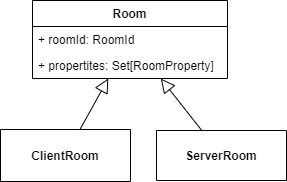
\includegraphics[scale=0.7]{images/3-architecture/room-class-3.png}
	\caption{Room class diagram}
	\label{fig:room_classes}
\end{figure}


At the most abstract level, a room is an entity that owns an unique Id and some properties that describe the room itself (figure \ref{fig:room_classes}).
\\
This is the basic model shared beween clients and server that each model will extend.

\bigskip
\textit{ServerRoom}
\\
The server room is the one that will be used by the server side developer. It provides functionalities to communicate and interact with connected clients. Besides, as specified in server requirement 2.1, the room behavior can be defined by the developer according to the application custom logic.

\bigskip
\textit{ClientRoom}
\\
On the other hand, the client room is the room that a client side developer will use. This component is meant to provide an interface towards the server side room, so that the developer can both send and receive messages from it. Obsviously, it exposes functionalities to define custom behavior too, as specified in client requirement 9.

\section{Server architecture} \label{sec:server_arch}
The main components of the server side architecture are visible in figure \ref{fig:server_classes}. 

\begin{figure}[H]
	\centering
	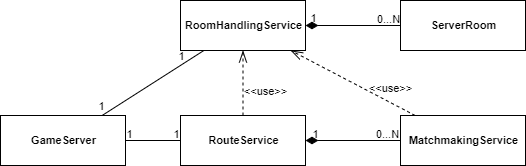
\includegraphics[scale=0.7]{images/3-architecture/server-architecture.png}
	\caption{Server architecture}
	\label{fig:server_classes}
\end{figure}

\bigskip
\textit{GameServer}
\\
The \texttt{GameServer} is the core component of the architecture and the starting point from where all the other components are created.
When dealing with the server module, a developer will mostly make use of its interface.

As shown in figure \ref{fig:server_classes}, it is connected to two other components: the \texttt{RouteService} and the \texttt{RoomHandlingService}.

\bigskip
\textit{RoomHandlingService}
\\
As the name suggests, the \texttt{RoomHandlingService} is the component used to manage rooms. It is meant to: 
\begin{itemize}
	\item Keep track of which rooms are currently active in the system
	\item Provide a way to interact with rooms (e.g creating and deleting rooms)
	\item Provide a way to define admissible types of room.
\end{itemize}

\bigskip
\textit{RouteService}
\\
This service is the classic routing module.
Every client request received by the gameserver using the request-response pattern is served by this component.
It defines routes (and associated handlers) that clients should contact when interacting with the server.
\\
Client requests can basically be split in two types:
\begin{itemize}
	\item Requests concerning rooms (e.g. connect to a room or retrieve available rooms). These requests are directly satisfied by the helping of the \texttt{RoomHandlingService}.
	\item Requests concerning matchmaking (e.g. join a matchmaking queue). These requests are fowarded and delegated to the right \texttt{MatchmakingService}, depending on the room type.
\end{itemize}

\bigskip
\textit{MatchmakingService}
\\
The \texttt{MatchmakingService} is the component that implements the matchmaking logic for a given type of room (i.e. adding clients to a queue, and eventually create fair groups according to some information about such clients). It needs to interact with the \texttt{RoomHandlingService} since, when a group of clients is formed, it must be created a room where those clients should connect to.


\section{Client Architecture}

\begin{figure}[H]
	\centering
	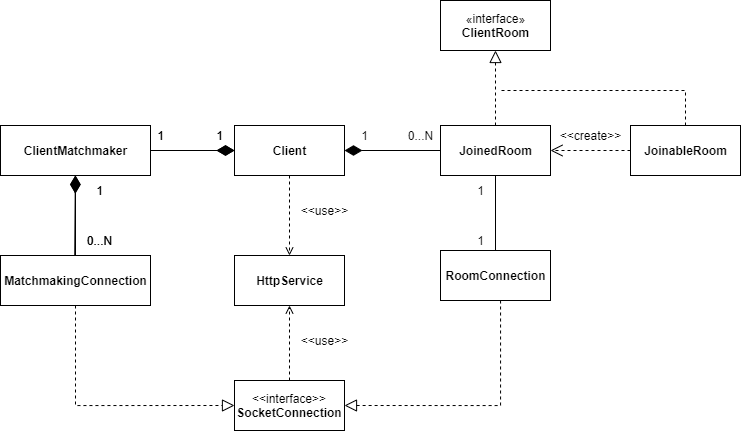
\includegraphics[scale=0.65]{images/3-architecture/client-architecture.png}
	\caption{Client architecture diagram}
	\label{fig:client_architecture}
\end{figure}

\section{Client-Server Interaction}
The requirements analysis led to the definition of three types of interaction between client and server:
\begin{enumerate}
	\item Client to GameServer \\
	This interaction takes place in those situations where the client makes a request to the server and waits for a specific response: for example getting the list of all rooms that can be joined. We decided to handle this kind of requests defining a REST protocol as shown in table
	 \ref{table:server_routes}.
	\begin{table}[]
		\begin{tabular}{p{2cm}p{4cm}p{2cm}p{5.5cm}}
			\textbf{Http Method} & \textbf{Path}	  & \textbf{Payload}  & \textbf{Result}                                                            		\\\\
			GET                  & /rooms             & filters           & get all the rooms that match the filters in the payload                        	\\\\
			GET                  & /rooms/:type       & filters           & get all the rooms with the given type (filtered by filters in the payload)     	\\\\
			GET                  & /rooms/:type/:id   & empty             & get the room with the given id searching among rooms of the given type         	\\\\
			POST                 & /rooms/:type       & options           & create a room of the given type with the option passed in the payload          	\\\\
			GET                  & /connection/:id    & websocket request & open a web socket connection with the room that has the given id               	\\\\
			GET                  & /matchmaking/:type & websocket request & open a web socket with the matchmaking service relative to the given room type 	\\\\
		\end{tabular}
		\caption{\label{table:server_routes} \textit{Server REST protocol for request-response interaction}}
	\end{table}
	\item  Client to Room \\
	In this case we are in a situation where a client wants to establish a connection with a given a room to both send and receive messages from it. The request-response pattern doesn't work here because now the communication channel must be full-duplex: the server can send data to the client even without a specific client request (for example if the room broadcasts a message to all connected clients).
	
	The chosen solution here is the websockets protocol since it provides the exact described behavior. Specifically, when a client wants to interact with a room, a websocket between that client and the server is created; the messages that the client sends through the socket are redirected to the room and the messages that the room wants to send to that client are forwarded through the socket. 
	
	Another consideration to make here is that clients can receive and send different types of messages through the socket: first of all they need to send a join message to notify the room that they want to enter; then they may want to send generic messages to that room (e.g. actions that affect the current game state) and eventually they'll want to leave the room, and so on \dots
	In order to identify this different kind of messages we decided to define a communication protocol that is used for messages in the websocket.
	
	
	\item Client to Matchmaking \\
	The last type of interaction is the one that takes place when a client wants to join the matchmaking queue for a given type of room. In this case the client asks the server to be added to the queue and waits to be grouped with other clients. We have decided to use websockets here too since when the client sends the request, the server response is not immediate. The communication must be kept open until the matchmaking service doesn't create the group of client to start the match. Only then the server can respond to the client with a message that contains the information to join the room that will host the game.
\end{enumerate}









